%Chapter "Introduction"
%
\chapter{Modelación Computacional}
\graphicspath{{img/mod_comp/}}

La modelación matemática y la simulación son herramientas matemáticas fundamentales en ciencia e ingeniería, y es válido afirmar que todo el mundo las usa (incluso aquellos que no se percatan de ello). La pregunta no es si usar estas herramienta o no, sino cómo usarlas de manera efectiva. Para tratar con la complejidad de un sistema de interés, los ingenieros y científicos usan versiones simplificadas del sistema, es decir, modelos del mismo \cite{book:velten-modeling}.

Es común encontrar palabras como sistema, modelo, y simulación muy a menudo en la literatura. Sin el interés de formalizar mucho en el asunto damos algunas definiciones para términos comúnmente encontrados:
\begin{itemize}
\item \textbf{Sistema:} Un sistema es un objeto o una colección de objetos de los cuáles queremos estudiar sus propiedades.

\item \textbf{Experimento:} Estimular un sistema para evaluar su respuesta.

\item \textbf{Modelo:} Abstracción de la realidad para un propósito específico.

\item \textbf{Simulación (experimento virtual):} Estimular un modelo del sistema de interés para evaluar su respuesta.
\end{itemize}

Podemos decir que el mejor modelo es el modelo más simple que sirve para entender un sistema y resolver problemas.

\section{Motivación}
Como un primer ejemplo, podemos pensar en el puente de Lymira, que es uno de los puentes en arco más antiguos del mundo\footnote{Se estima que el puente fue construido en el siglo III d.C.}. 
\begin{figure}[H]
\centering
\includegraphics[width=10cm]{{Bridge_near_Limyra._Pic_04}.jpg}\\
\includegraphics[width=10cm]{{Ubicacion_puente}.png}
\caption{(\textbf{Arriba}) Foto del puente de Lymira en la actualidad. (\textbf{Abajo}) Ubicación del puente, en la actual Turquía.}
\end{figure}

La \cref{fig:puente} muestra un esquema de la geometría simplificada para una sección de un puente similar al mostrado anteriormente. También muestra los contornos de desplazamiento verticales obtenidos por el método de los elementos finitos bajo la aplicación de una carga uniforme y vertical en la superficie del puente.
\begin{figure}[H] 
\centering
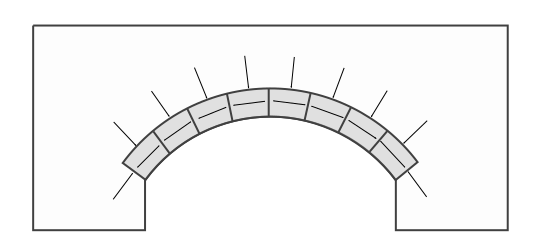
\includegraphics[height=5 cm]{Arco.pdf}\\
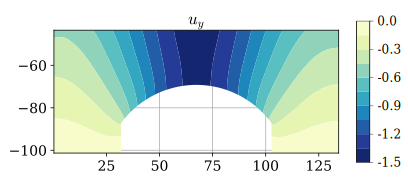
\includegraphics[height=6 cm]{Arco_vertical_disp.pdf}
\caption{Un arco colecta las cargas verticales y las convierte en cargas laterales. Estas cargas laterales van a través del arco y son soportadas por el contrafuerte \cite{book:gordon-structures}. En la parte inferior vemos el resultado de una simulación por elementos finitos, los contornos representan el desplazamiento vertical en cada punto.}
\label{fig:puente}
\end{figure}


\section{Ejemplos}

\subsection{Caída libre de un paracaidista}
Como primer ejemplo, estudiemos la velo caída libre de un paracaidista. Despreciaremos la velocidad horizontal y consideraremos que la velocidad vertical inicial es cero. Para encontrar las ecuaciones de movimiento partamos de un diagrama de cuerpo libre.
\begin{figure}[h] 
\centering
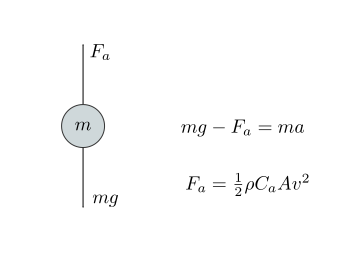
\includegraphics[width=4 in]{caida_libre.pdf}
\caption{Diagrama de cuerpo libre para una partícula de masa \(m\) que cae en bajo la resistencia de un fluido.}
\label{fig:caida_libre}
\end{figure}

La resistencia del aire está dada por
\[F_a = \frac{1}{2}\rho C_a A v^2\, ,\]
con \(\rho\) la densidad del fluido, \(C_a\) el coeficiente de arrastre, \(A\) la sección transversal y \(v\) la velocidad. Por tanto, tenemos la siguiente ecuación de movimiento
\[\dv{v}{t} = g - \frac{1}{2}\frac{\rho C_a A}{m} v^2\, .\]

A diferencia de la caída en la ausencia de un fluido, en este caso se tiene una ``velocidad terminal" (\(v_\infty\)), es decir, una velocidad máxima. Esto implica que la aceleración debe ser cero,
\[\dv{v_\infty}{t} = 0\, ,\]
y por tanto
\[g = \frac{1}{2}\frac{\rho C_a A}{m} v^2_\infty\, ,\quad \text{o}\quad v_\infty = \sqrt{\frac{2 m g}{\rho C_a A}} \, .\]

Podemos, entonces, reescribir la ecuación diferencial como
\[\dv{v}{t} = g\left(1 - \frac{v^2}{v_\infty^2}\right)\, ,\]
e integrando tenemos
\[\int_0^v \frac{\dd{v}}{\left(1 - \frac{v^2}{v_\infty^2}\right)} = \int_0^t g \dd{t}\, ,\]
y luego de una manipulación algebraica, obtenemos
\[v(t) = v_\infty \tanh\left(\frac{gt}{v_\infty}\right)\, .\]

Tomemos los siguientes parámetros: \(\rho = 1.22\, \unit{kg/m^3}\), \(g=9.81\, \unit{m/s^2}\), \(C_a = 1.2\), \(A = 0.43\, \unit{m^2}\) , y
\(m = 80\, \unit{kg}\). Esto nos da una velocidad terminal
\[v_\infty = 49.94\, \unit{m/s} = 179.76\, \unit{km/h}\, ,\]
y la rapidez como función del tiempo sería
\[v(t) = 49.94\, \tanh(0.196\, t)\, \unit{m/s}\, .\]

La siguiente figura muestra esta función entre 0 y 10 segundos
\begin{figure}[H] 
\centering
\includegraphics[width=4 in]{velocidad_caida_libre.pdf}
\caption{Rapidez en función del tiempo para un paracaidista en caída libre.}
\label{fig:vel_caida_libre}
\end{figure}

Ahora, supongamos que no sabemos cómo resolver la ecuación diferencial. Podemos usar el método de Euler para encontrar su solución numéricamente. El método de Euler se basa en aproximar la solución a partir de la solución en un instante actual usando una línea recta que pasa por el punto actual y tiene pendiente igual a la derivada evaluada en dicho punto. La idea se ilustra gráficamente a continuación.
\begin{figure}[H] 
\centering
\includegraphics[width=4 in]{euler.pdf}
\caption{Esquema del método de Euler. El valor de velocidad para \(t +\Delta t\) se calcula a partir del valor para \(t\) y la pendiente de la recta es igual a la derivada evaluada en \(t\).}
\label{fig:metodo_euler}
\end{figure}

En nuestro ejemplo tenemos la siguiente ecuación diferencial
\[v'(t) \equiv \dv{v}{t} = g\left(1 - \frac{v^2(t)}{v_\infty^2}\right)\, ,\]
y usando la ecuación de la pendiente tenemos que
\[v'(t) \approx \frac{v(t + \Delta t) - v(t)}{(t+\Delta t) - (t)}\, ,\]
que resulta en
\[v(t + \Delta t) \approx v(t) + \Delta t\, v'(t)\, ,\]
y remplazando la ecuación diferencial, obtendríamos la siguiente formula iterativa.
\[ v(t + \Delta t) \approx v(t) + \Delta t\, g\left(1 - \frac{v^2(t)}{v_\infty^2}\right)\, .\]

Esto nos permitiría resolver la ecuación de forma iterativa en una hoja de cálculo o con algún lenguaje de programación. A continuación se muestra el código en Python para este problema.
\begin{listing}[H]
    \begin{minted}[mathescape,
               gobble=8,
               frame=lines,
               framesep=2mm]{python}
        import numpy as np

        rho = 1.22 # kg/m**3
        g = 9.81 # m/s**2
        Ca = 1.2
        A = 0.43 # m**2
        m = 80.0 # kg
        v_inf = np.sqrt(2*m*g/(rho * Ca * A))
        t = np.linspace(0, 10, 10)
        dt = t[1] - t[0]
        niter = len(t)
        v = np.zeros(niter)
        for cont in range(1, niter):
            v[cont] = v[cont - 1] + dt * g * (1 - v[cont - 1]**2/v_inf**2)
    \end{minted}
    \caption{Método de Euler para el problema de caída libre de un paracaidista.}
    \label{lst:euler}
\end{listing}

La \cref{fig:euler_caida} presenta la solución por este método y la compara con la solución analítica.
\begin{figure}[H] 
\centering
\includegraphics[width=4 in]{euler_caida.pdf}
\caption{Rapidez en función del tiempo para un paracaidista en caída libre calculada con el método de Euler.}
\label{fig:euler_caida}
\end{figure}

\subsection{Vibración en una cuerda}
En este ejemplo queremos estudiar la vibración en una cuerda con pequeñas amplitudes. Para ello, partimos de la ecuación de conservación del moméntum lineal (segunda ley de Newton). Asumiremos que la cuerda es homogénea y la tensión experimentada es la misma a lo largo de ella. Tomemos un elemento diferencial de la cuerda como se muestra en la siguiente figura.
\begin{figure}[H] 
\centering
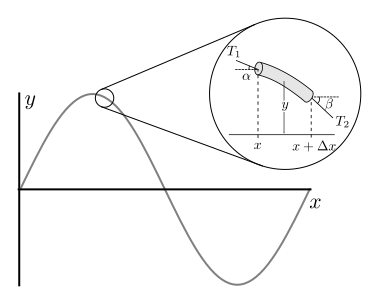
\includegraphics[height=8 cm]{cuerda.pdf}
\caption{Fuerzas actuando sobre un elemento diferencial de una cuerda de longitud \(\Delta m\).}
\label{fig:cuerda}
\end{figure}

Horizontalmente tenemos
\begin{align*}
&T_{1x} = T_1 \cos\alpha \approx T\\
&T_{2x} = T_2 \cos\beta \approx T\, .
\end{align*}

Si los ángulos son pequeños las fuerzas horizontales son iguales y su sumatoria es cero. Verticalmente, tenemos entonces
\[\sum F_y = T_{1y} - T_{2y} = - T_2\sin\beta + T_1\sin\alpha = \Delta m\, a \approx \mu \Delta x \pdv[2]{y}{t}\, ,\]
en donde tomamos que la masa del elemento diferencial \(\Delta m = \mu \Delta x\), siendo \(\mu\) la densidad de masa por unidad de longitud. Si dividimos por \(T\) y remplazamos la primera ecuación  para \(T\), obtenemos
\[\frac{\mu \Delta x}{T}\pdv[2]{y}{t} = -\frac{T_2 \sin\beta}{T_2\cos\beta} + \frac{T_1\sin\alpha}{T_1\cos\alpha} = -\tan\beta + \tan\alpha\, .\]

Y sabemos que las tangentes de estos ángulos son iguales a las pendientes, es decir,
\[\frac{1}{\Delta x}\left(\left.\pdv{y}{x}\right|_{x + \Delta x} - \left.\pdv{y}{x}\right|_{x}\right) = \frac{\mu}{T}\pdv[2]{y}{t}\, .\]

En el límite \(\Delta x \rightarrow 0\), tenemos
\[\pdv[2]{y(x, t)}{x} = \frac{1}{c^2}\pdv[2]{y(x, t)}{t}\, ,\]
con \(c^2 = T/\mu\), la velocidad de propagación de la onda. Esta velocidad es directamente proporcional a la raíz cuadrada de la tensión en la cuerda e inversamente proporcional a la raíz cuadrada de la densidad lineal de masa.

A este tipo de ecuaciones se le denomina ``ecuaciones en derivadas parciales'' porque ecuación incluye la incógnita, \(y(x, t)\), así como sus derivadas parciales. A fijar la cuerda en ambos extremos denominamos condiciones de frontera, y a conocer su configuración inicial (posición y velocidad) condiciones iniciales. Para este problema se cuenta con una solución analítica, sin embargo, usaremos una estrategia numérica llamada ``diferencias finitas''.

Este método aproxima las derivadas por medio de \emph{diferencias} de la función en puntos adyacentes, y se asemeja a la definición de derivada usando el límite, es decir
\[\pdv[2]{u(x, t)}{x} \approx \frac{u_{x + 1}^t - 2 u_x^t + u_{x-1}^t}{\Delta x^2}\, ,\]
y
\[\pdv[2]{u(x, t)}{t} \approx \frac{u_x^{t + 2} - 2 u_x^{t + 1} + u_x^t}{\Delta t^2}\, ,\]
en donde los subíndices se refieren a una discretización en el espacio (\(x\)) y los superíndices se refieren a una discretización en el tiempo (\(t\)).

Usando estas aproximaciones en la ecuación diferencial, tenemos
\[\frac{y_{x + 1}^t - 2 y_x^t + y_{x-1}^t}{\Delta x^2} = \frac{1}{c^2}\left(\frac{y_x^{t + 1} - 2 y_x^t + y_x^{t - 1}}{\Delta t^2}\right)\, ,\]
y despejando \(y_x^{t+1}\),
\begin{equation}
  y_x^{t + 2} = 2 y_x^{t + 1} - y_x^t + \frac{c^2 \Delta t^2}{\Delta x^2}\left[y_{x+1}^t - 2y_x^t + y_{x-1}^t\right]\, ,
\end{equation}
y podemos ver que tenemos una fórmula recursiva para obtener la solución en el tiempo \(t + 2\) a partir de la solución en dos tiempos anteriores.

Esta fórmula no funciona para la primera iteración, pues requiere conocer la solución en un instante anterior al tiempo inicial (\(y_x^{-1}\)), sin embargo podemos usar la condición inicial para la primera derivada de \(y\) para obtener
\[y_x^1 = y_x^0 - \Delta y'_x - \frac{1}{2}\frac{c^2 \Delta t^2}{\delta x^2}\left[y_{x+1}^0 - 2y_x^0 + y_{x-1}^0\right]\, .\]